% Options for packages loaded elsewhere
\PassOptionsToPackage{unicode}{hyperref}
\PassOptionsToPackage{hyphens}{url}
%
\documentclass[
  11pt,
  ignorenonframetext,
]{beamer}
\usepackage{pgfpages}
\setbeamertemplate{caption}[numbered]
\setbeamertemplate{caption label separator}{: }
\setbeamercolor{caption name}{fg=normal text.fg}
\beamertemplatenavigationsymbolsempty
% Prevent slide breaks in the middle of a paragraph
\widowpenalties 1 10000
\raggedbottom
\setbeamertemplate{part page}{
  \centering
  \begin{beamercolorbox}[sep=16pt,center]{part title}
    \usebeamerfont{part title}\insertpart\par
  \end{beamercolorbox}
}
\setbeamertemplate{section page}{
  \centering
  \begin{beamercolorbox}[sep=12pt,center]{part title}
    \usebeamerfont{section title}\insertsection\par
  \end{beamercolorbox}
}
\setbeamertemplate{subsection page}{
  \centering
  \begin{beamercolorbox}[sep=8pt,center]{part title}
    \usebeamerfont{subsection title}\insertsubsection\par
  \end{beamercolorbox}
}
\AtBeginPart{
  \frame{\partpage}
}
\AtBeginSection{
  \ifbibliography
  \else
    \frame{\sectionpage}
  \fi
}
\AtBeginSubsection{
  \frame{\subsectionpage}
}
\usepackage{amsmath,amssymb}
\usepackage{lmodern}
\usepackage{iftex}
\ifPDFTeX
  \usepackage[T1]{fontenc}
  \usepackage[utf8]{inputenc}
  \usepackage{textcomp} % provide euro and other symbols
\else % if luatex or xetex
  \usepackage{unicode-math}
  \defaultfontfeatures{Scale=MatchLowercase}
  \defaultfontfeatures[\rmfamily]{Ligatures=TeX,Scale=1}
\fi
\usetheme[]{metropolis}
% Use upquote if available, for straight quotes in verbatim environments
\IfFileExists{upquote.sty}{\usepackage{upquote}}{}
\IfFileExists{microtype.sty}{% use microtype if available
  \usepackage[]{microtype}
  \UseMicrotypeSet[protrusion]{basicmath} % disable protrusion for tt fonts
}{}
\makeatletter
\@ifundefined{KOMAClassName}{% if non-KOMA class
  \IfFileExists{parskip.sty}{%
    \usepackage{parskip}
  }{% else
    \setlength{\parindent}{0pt}
    \setlength{\parskip}{6pt plus 2pt minus 1pt}}
}{% if KOMA class
  \KOMAoptions{parskip=half}}
\makeatother
\usepackage{xcolor}
\newif\ifbibliography
\usepackage{color}
\usepackage{fancyvrb}
\newcommand{\VerbBar}{|}
\newcommand{\VERB}{\Verb[commandchars=\\\{\}]}
\DefineVerbatimEnvironment{Highlighting}{Verbatim}{commandchars=\\\{\}}
% Add ',fontsize=\small' for more characters per line
\newenvironment{Shaded}{}{}
\newcommand{\AlertTok}[1]{\textcolor[rgb]{1.00,0.00,0.00}{\textbf{#1}}}
\newcommand{\AnnotationTok}[1]{\textcolor[rgb]{0.38,0.63,0.69}{\textbf{\textit{#1}}}}
\newcommand{\AttributeTok}[1]{\textcolor[rgb]{0.49,0.56,0.16}{#1}}
\newcommand{\BaseNTok}[1]{\textcolor[rgb]{0.25,0.63,0.44}{#1}}
\newcommand{\BuiltInTok}[1]{\textcolor[rgb]{0.00,0.50,0.00}{#1}}
\newcommand{\CharTok}[1]{\textcolor[rgb]{0.25,0.44,0.63}{#1}}
\newcommand{\CommentTok}[1]{\textcolor[rgb]{0.38,0.63,0.69}{\textit{#1}}}
\newcommand{\CommentVarTok}[1]{\textcolor[rgb]{0.38,0.63,0.69}{\textbf{\textit{#1}}}}
\newcommand{\ConstantTok}[1]{\textcolor[rgb]{0.53,0.00,0.00}{#1}}
\newcommand{\ControlFlowTok}[1]{\textcolor[rgb]{0.00,0.44,0.13}{\textbf{#1}}}
\newcommand{\DataTypeTok}[1]{\textcolor[rgb]{0.56,0.13,0.00}{#1}}
\newcommand{\DecValTok}[1]{\textcolor[rgb]{0.25,0.63,0.44}{#1}}
\newcommand{\DocumentationTok}[1]{\textcolor[rgb]{0.73,0.13,0.13}{\textit{#1}}}
\newcommand{\ErrorTok}[1]{\textcolor[rgb]{1.00,0.00,0.00}{\textbf{#1}}}
\newcommand{\ExtensionTok}[1]{#1}
\newcommand{\FloatTok}[1]{\textcolor[rgb]{0.25,0.63,0.44}{#1}}
\newcommand{\FunctionTok}[1]{\textcolor[rgb]{0.02,0.16,0.49}{#1}}
\newcommand{\ImportTok}[1]{\textcolor[rgb]{0.00,0.50,0.00}{\textbf{#1}}}
\newcommand{\InformationTok}[1]{\textcolor[rgb]{0.38,0.63,0.69}{\textbf{\textit{#1}}}}
\newcommand{\KeywordTok}[1]{\textcolor[rgb]{0.00,0.44,0.13}{\textbf{#1}}}
\newcommand{\NormalTok}[1]{#1}
\newcommand{\OperatorTok}[1]{\textcolor[rgb]{0.40,0.40,0.40}{#1}}
\newcommand{\OtherTok}[1]{\textcolor[rgb]{0.00,0.44,0.13}{#1}}
\newcommand{\PreprocessorTok}[1]{\textcolor[rgb]{0.74,0.48,0.00}{#1}}
\newcommand{\RegionMarkerTok}[1]{#1}
\newcommand{\SpecialCharTok}[1]{\textcolor[rgb]{0.25,0.44,0.63}{#1}}
\newcommand{\SpecialStringTok}[1]{\textcolor[rgb]{0.73,0.40,0.53}{#1}}
\newcommand{\StringTok}[1]{\textcolor[rgb]{0.25,0.44,0.63}{#1}}
\newcommand{\VariableTok}[1]{\textcolor[rgb]{0.10,0.09,0.49}{#1}}
\newcommand{\VerbatimStringTok}[1]{\textcolor[rgb]{0.25,0.44,0.63}{#1}}
\newcommand{\WarningTok}[1]{\textcolor[rgb]{0.38,0.63,0.69}{\textbf{\textit{#1}}}}
\usepackage{longtable,booktabs,array}
\usepackage{calc} % for calculating minipage widths
\usepackage{caption}
% Make caption package work with longtable
\makeatletter
\def\fnum@table{\tablename~\thetable}
\makeatother
\usepackage{graphicx}
\makeatletter
\def\maxwidth{\ifdim\Gin@nat@width>\linewidth\linewidth\else\Gin@nat@width\fi}
\def\maxheight{\ifdim\Gin@nat@height>\textheight\textheight\else\Gin@nat@height\fi}
\makeatother
% Scale images if necessary, so that they will not overflow the page
% margins by default, and it is still possible to overwrite the defaults
% using explicit options in \includegraphics[width, height, ...]{}
\setkeys{Gin}{width=\maxwidth,height=\maxheight,keepaspectratio}
% Set default figure placement to htbp
\makeatletter
\def\fps@figure{htbp}
\makeatother
\setlength{\emergencystretch}{3em} % prevent overfull lines
\providecommand{\tightlist}{%
  \setlength{\itemsep}{0pt}\setlength{\parskip}{0pt}}
\setcounter{secnumdepth}{-\maxdimen} % remove section numbering
\ifLuaTeX
  \usepackage{selnolig}  % disable illegal ligatures
\fi
\IfFileExists{bookmark.sty}{\usepackage{bookmark}}{\usepackage{hyperref}}
\IfFileExists{xurl.sty}{\usepackage{xurl}}{} % add URL line breaks if available
\urlstyle{same} % disable monospaced font for URLs
\hypersetup{
  pdftitle={Análisis de la asociación espacial},
  pdfauthor={Gerardo Martín},
  hidelinks,
  pdfcreator={LaTeX via pandoc}}

\title{Análisis de la asociación espacial}
\subtitle{Regresión}
\author{Gerardo Martín}
\date{2022-06-29}

\begin{document}
\frame{\titlepage}

\begin{frame}{Diferencias y similitudes con correlación}
\protect\hypertarget{diferencias-y-similitudes-con-correlaciuxf3n}{}
\begin{itemize}
\item
  Correlación mide dependencia lineal entre dos fenómenos
\item
  No hay causa - efecto:

  \begin{itemize}
  \tightlist
  \item
    \(\mathrm{cov}(X, Y) = \mathrm{cov}(Y, X)\)
  \end{itemize}
\item
  No permite estimar cambio de una con respecto de la otra
\item
  Regresión, sí se asume causa y efecto:

  \begin{itemize}
  \tightlist
  \item
    \(y(x) = a + bx\)
  \end{itemize}
\end{itemize}
\end{frame}

\begin{frame}{Diferencias y similitudes con correlación}
\protect\hypertarget{diferencias-y-similitudes-con-correlaciuxf3n-1}{}
\begin{itemize}
\item
  Correlación, sólo conocemos \(r\), ó \(\rho\) (correlación de
  Spearman)

  \begin{itemize}
  \item
    Signo de \(r\) indica si una disminuye ó aumenta en relación a la
    otra
  \item
    \(P\) indica probabilidad de que \(r = 0\)
  \end{itemize}
\item
  Regresión

  \begin{itemize}
  \item
    Coeficientes \(a\) y \(b\) cuantifican relación entre \(x\) y \(y\)
  \item
    \(a\), valor de \(y\) cuando \(x = 0\)
  \item
    \(b\), aumento ó disminución de \(y\) cuando \(x\) aumenta en 1
    unidad
  \item
    \(R^2\), cuadrado del coeficiete de correlación \(r\)
  \end{itemize}
\end{itemize}
\end{frame}

\begin{frame}{Diferencias gráficas}
\protect\hypertarget{diferencias-gruxe1ficas}{}
\begin{center}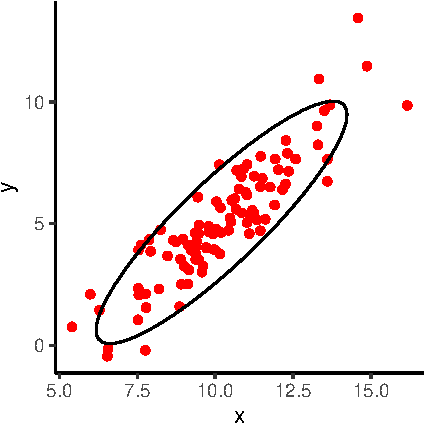
\includegraphics{Regresion_files/figure-beamer/unnamed-chunk-1-1} \end{center}
\end{frame}

\begin{frame}{Diferencias gráficas}
\protect\hypertarget{diferencias-gruxe1ficas-1}{}
\begin{center}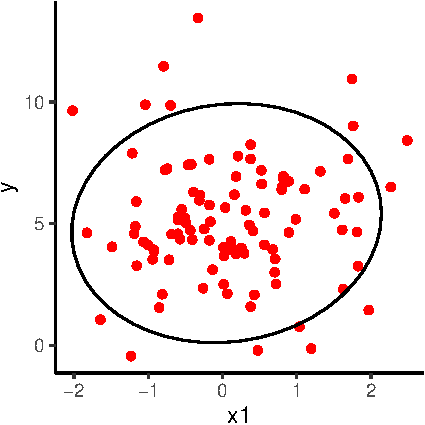
\includegraphics{Regresion_files/figure-beamer/unnamed-chunk-2-1} \end{center}
\end{frame}

\begin{frame}{Diferencias gráficas}
\protect\hypertarget{diferencias-gruxe1ficas-2}{}
\begin{center}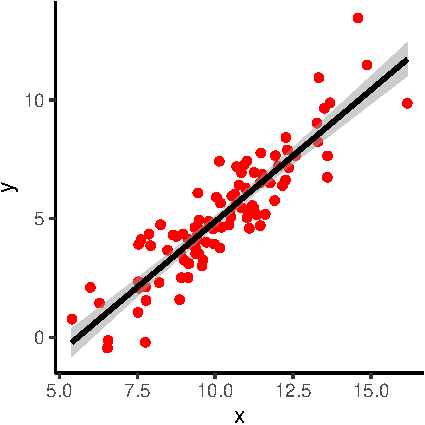
\includegraphics{Regresion_files/figure-beamer/unnamed-chunk-3-1} \end{center}
\end{frame}

\begin{frame}{Diferencias gráficas}
\protect\hypertarget{diferencias-gruxe1ficas-3}{}
\begin{center}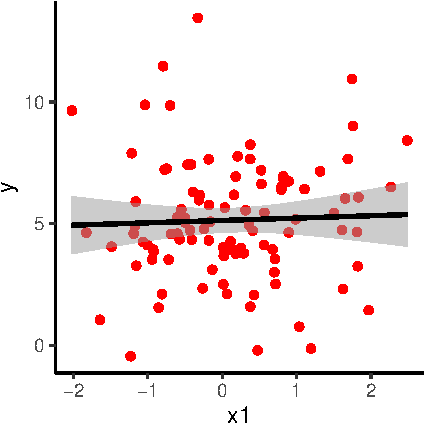
\includegraphics{Regresion_files/figure-beamer/unnamed-chunk-4-1} \end{center}
\end{frame}

\begin{frame}{Significato de parámetros}
\protect\hypertarget{significato-de-paruxe1metros}{}
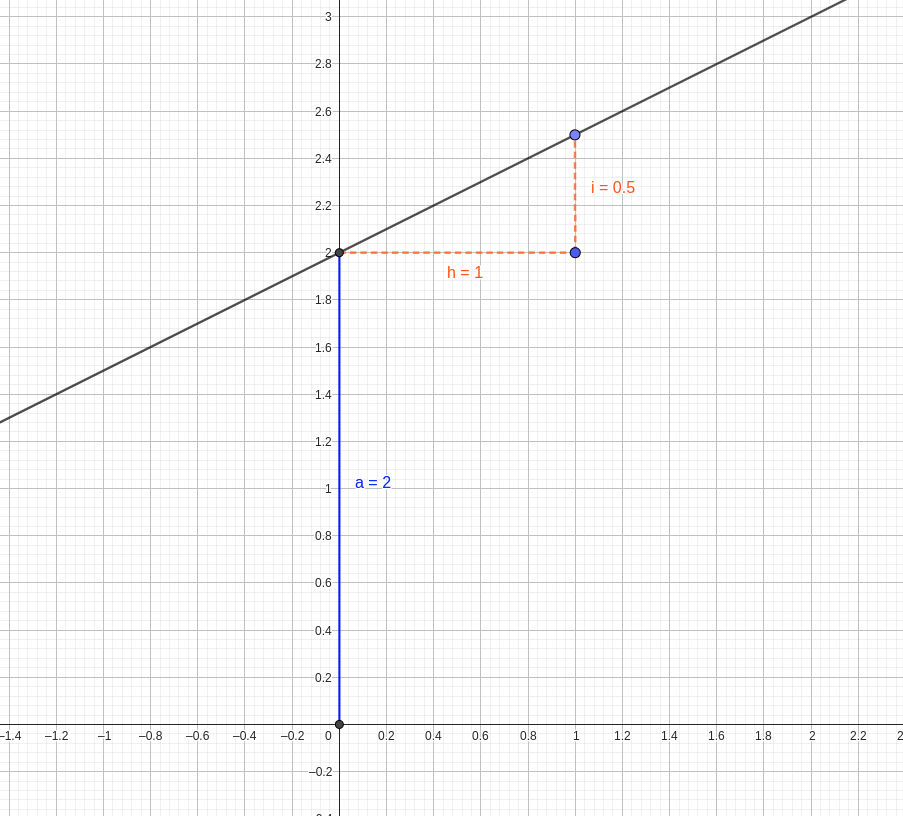
\includegraphics{La-recta.png}
\end{frame}

\begin{frame}{Significado de parámetros}
\protect\hypertarget{significado-de-paruxe1metros}{}
\[y(x) = a + bx\]

\begin{itemize}
\item
  \(a\) = 2
\item
  \(b = i/h = 0.5\)
\end{itemize}

\[y(x) = 2 + 0.5 x\]
\end{frame}

\begin{frame}[fragile]{Implementando en R}
\protect\hypertarget{implementando-en-r}{}
\begin{itemize}
\item
  Función nativa para estimar \(a\), \(b\) y \(R^2\), \texttt{lm}
\item
  Hipótesis que queremos rechazar, \(x\) no afecta a \(y\)

  \begin{itemize}
  \tightlist
  \item
    \(a \neq 0\), \(b \neq 0\)
  \end{itemize}
\item
  Uso:
\end{itemize}

\begin{Shaded}
\begin{Highlighting}[]
\FunctionTok{lm}\NormalTok{(x }\SpecialCharTok{\textasciitilde{}}\NormalTok{ y, }\AttributeTok{data =}\NormalTok{ df}\FloatTok{.1}\NormalTok{) }\CommentTok{\#df.1 es tabla que contiene datos de x y y}
\end{Highlighting}
\end{Shaded}
\end{frame}

\begin{frame}[fragile]{Implementando en R}
\protect\hypertarget{implementando-en-r-1}{}
\begin{Shaded}
\begin{Highlighting}[]
\NormalTok{reg.lin }\OtherTok{\textless{}{-}} \FunctionTok{lm}\NormalTok{(y }\SpecialCharTok{\textasciitilde{}}\NormalTok{ x, }\AttributeTok{data =}\NormalTok{ df}\FloatTok{.1}\NormalTok{)}
\FunctionTok{summary}\NormalTok{(reg.lin)}
\end{Highlighting}
\end{Shaded}

\begin{verbatim}
## 
## Call:
## lm(formula = y ~ x, data = df.1)
## 
## Residuals:
##     Min      1Q  Median      3Q     Max 
## -2.6090 -0.8366 -0.0884  0.6772  3.4914 
## 
## Coefficients:
##             Estimate Std. Error t value Pr(>|t|)    
## (Intercept) -6.20626    0.58606  -10.59   <2e-16 ***
## x            1.10859    0.05621   19.72   <2e-16 ***
## ---
## Signif. codes:  0 '***' 0.001 '**' 0.01 '*' 0.05 '.' 0.1 ' ' 1
## 
## Residual standard error: 1.112 on 98 degrees of freedom
## Multiple R-squared:  0.7987, Adjusted R-squared:  0.7967 
## F-statistic: 388.9 on 1 and 98 DF,  p-value: < 2.2e-16
\end{verbatim}
\end{frame}

\begin{frame}[fragile]{Implementando en R}
\protect\hypertarget{implementando-en-r-2}{}
\textbf{Columnas}

\begin{itemize}
\item
  \texttt{Estimate} contiene el valor estimado
\item
  \texttt{Pr(\textgreater{}\textbar{}t\textbar{})} es la probabilidad de
  que \(a = 0\) ó \(b=0\)
\end{itemize}

\textbf{Filas}

\begin{itemize}
\item
  \(a = \mathtt{(Intercept)}\)
\item
  \(b = \mathtt{x}\)
\item
  \(R^2 = \mathtt{Adjusted\ R-squared}\)
\end{itemize}
\end{frame}

\begin{frame}[fragile]{Implementando en R}
\protect\hypertarget{implementando-en-r-3}{}
\begin{Shaded}
\begin{Highlighting}[]
\NormalTok{reg.lin1 }\OtherTok{\textless{}{-}} \FunctionTok{lm}\NormalTok{(y }\SpecialCharTok{\textasciitilde{}}\NormalTok{ x1, }\AttributeTok{data =}\NormalTok{ df}\FloatTok{.1}\NormalTok{)}
\FunctionTok{summary}\NormalTok{(reg.lin1)}
\end{Highlighting}
\end{Shaded}

\begin{verbatim}
## 
## Call:
## lm(formula = y ~ x1, data = df.1)
## 
## Residuals:
##     Min      1Q  Median      3Q     Max 
## -5.4589 -1.2876 -0.2732  1.3428  8.3563 
## 
## Coefficients:
##             Estimate Std. Error t value Pr(>|t|)    
## (Intercept)  5.13185    0.24895  20.614   <2e-16 ***
## x1           0.09689    0.25581   0.379    0.706    
## ---
## Signif. codes:  0 '***' 0.001 '**' 0.01 '*' 0.05 '.' 0.1 ' ' 1
## 
## Residual standard error: 2.476 on 98 degrees of freedom
## Multiple R-squared:  0.001462,   Adjusted R-squared:  -0.008727 
## F-statistic: 0.1435 on 1 and 98 DF,  p-value: 0.7057
\end{verbatim}
\end{frame}

\begin{frame}{Regresión lineal con datos espaciales}
\protect\hypertarget{regresiuxf3n-lineal-con-datos-espaciales}{}
Al igual que en correlación, debemos:

\begin{enumerate}
\item
  Extraer
\item
  Añadir a base de coordenadas
\item
  Ajustar
\item
  Interpretar
\item
  Predecir
\end{enumerate}
\end{frame}

\begin{frame}{Regresión con datos espaciales}
\protect\hypertarget{regresiuxf3n-con-datos-espaciales}{}
Retomaremos el ejemplo de la correlación espacial:

\begin{longtable}[]{@{}rrr@{}}
\caption{Primeras seis filas de una base de datos de mediciones
colectadas en campo.}\tabularnewline
\toprule()
x & y & mediciones \\
\midrule()
\endfirsthead
\toprule()
x & y & mediciones \\
\midrule()
\endhead
-102.7928 & 29.57881 & 49.62024 \\
-103.6011 & 27.38053 & 41.14992 \\
-104.5670 & 25.53772 & 137.04156 \\
-101.8276 & 29.87109 & 51.70786 \\
-100.5730 & 27.40428 & 103.70981 \\
-101.0474 & 29.20245 & 75.43274 \\
\bottomrule()
\end{longtable}
\end{frame}

\begin{frame}{Gráfico de los valores colectados}
\protect\hypertarget{gruxe1fico-de-los-valores-colectados}{}
\begin{figure}

{\centering 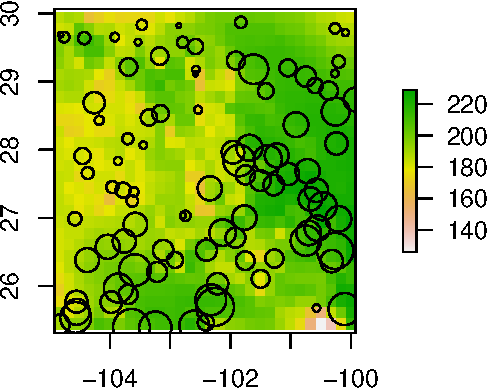
\includegraphics{Regresion_files/figure-beamer/unnamed-chunk-9-1} 

}

\caption{Diámetro de burbujas indica magnitud}\label{fig:unnamed-chunk-9}
\end{figure}
\end{frame}

\begin{frame}[fragile]{Extrayendo valores de capas raster}
\protect\hypertarget{extrayendo-valores-de-capas-raster}{}
\begin{Shaded}
\begin{Highlighting}[]
\NormalTok{valores.capas }\OtherTok{\textless{}{-}} \FunctionTok{extract}\NormalTok{(r, puntos[, }\FunctionTok{c}\NormalTok{(}\StringTok{"x"}\NormalTok{, }\StringTok{"y"}\NormalTok{)])}
\NormalTok{puntos }\OtherTok{\textless{}{-}} \FunctionTok{data.frame}\NormalTok{(puntos, valores.capas)}
\end{Highlighting}
\end{Shaded}
\end{frame}

\begin{frame}{Valores extraídos de capa raster}
\protect\hypertarget{valores-extrauxeddos-de-capa-raster}{}
\begin{longtable}[]{@{}rrrrrr@{}}
\toprule()
x & y & mediciones & Var.1 & Var.2 & Var.3 \\
\midrule()
\endhead
-102.7928 & 29.57881 & 49.62024 & 199 & 106 & 161 \\
-103.6011 & 27.38053 & 41.14992 & 179 & 105 & 143 \\
-104.5670 & 25.53772 & 137.04156 & 187 & 126 & 193 \\
-101.8276 & 29.87109 & 51.70786 & 203 & 105 & 149 \\
-100.5730 & 27.40428 & 103.70981 & 224 & 135 & 143 \\
-101.0474 & 29.20245 & 75.43274 & 213 & 121 & 131 \\
-102.5358 & 28.58792 & 35.05952 & 174 & 101 & 132 \\
-101.4132 & 28.86275 & 69.94669 & 209 & 125 & 134 \\
-102.3974 & 26.52351 & 92.91473 & 211 & 134 & 153 \\
-102.6020 & 25.42059 & 131.78474 & 218 & 147 & 148 \\
\bottomrule()
\end{longtable}
\end{frame}

\begin{frame}[fragile]{Ajustando el modelo lineal}
\protect\hypertarget{ajustando-el-modelo-lineal}{}
Con base en análisis de correlación sabemos que es más probable que
\texttt{Var.2} explique las mediciones:

\begin{Shaded}
\begin{Highlighting}[]
\NormalTok{m1 }\OtherTok{\textless{}{-}} \FunctionTok{lm}\NormalTok{(mediciones }\SpecialCharTok{\textasciitilde{}}\NormalTok{ Var}\FloatTok{.2}\NormalTok{, puntos)}
\end{Highlighting}
\end{Shaded}
\end{frame}

\begin{frame}[fragile]{Ajustando el modelo lineal}
\protect\hypertarget{ajustando-el-modelo-lineal-1}{}
\begin{Shaded}
\begin{Highlighting}[]
\FunctionTok{summary}\NormalTok{(m1)}
\end{Highlighting}
\end{Shaded}

\begin{verbatim}
## 
## Call:
## lm(formula = mediciones ~ Var.2, data = puntos)
## 
## Residuals:
##     Min      1Q  Median      3Q     Max 
## -70.751 -13.179  -0.278  13.347  56.566 
## 
## Coefficients:
##              Estimate Std. Error t value Pr(>|t|)    
## (Intercept) -160.5896    18.0366  -8.904 3.12e-14 ***
## Var.2          2.0531     0.1505  13.641  < 2e-16 ***
## ---
## Signif. codes:  0 '***' 0.001 '**' 0.01 '*' 0.05 '.' 0.1 ' ' 1
## 
## Residual standard error: 22.4 on 97 degrees of freedom
## Multiple R-squared:  0.6573, Adjusted R-squared:  0.6538 
## F-statistic: 186.1 on 1 and 97 DF,  p-value: < 2.2e-16
\end{verbatim}
\end{frame}

\begin{frame}[fragile]{Predicción espacial}
\protect\hypertarget{predicciuxf3n-espacial}{}
Necesitamos crear base con valores para predecir:

\begin{Shaded}
\begin{Highlighting}[]
\NormalTok{val.nuevos }\OtherTok{\textless{}{-}} \FunctionTok{data.frame}\NormalTok{(}\FunctionTok{rasterToPoints}\NormalTok{(r))}
\NormalTok{preds }\OtherTok{\textless{}{-}} \FunctionTok{predict}\NormalTok{(m1, val.nuevos)}
\NormalTok{preds.r }\OtherTok{\textless{}{-}} \FunctionTok{rasterFromXYZ}\NormalTok{(}\FunctionTok{data.frame}\NormalTok{(val.nuevos[, }\FunctionTok{c}\NormalTok{(}\StringTok{"x"}\NormalTok{, }\StringTok{"y"}\NormalTok{)], preds))}
\end{Highlighting}
\end{Shaded}
\end{frame}

\begin{frame}{Gráfico de la predicción}
\protect\hypertarget{gruxe1fico-de-la-predicciuxf3n}{}
\begin{center}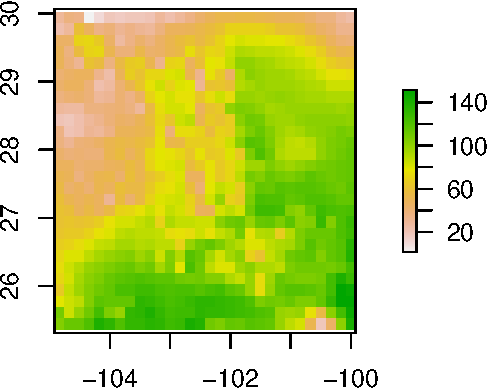
\includegraphics{Regresion_files/figure-beamer/unnamed-chunk-15-1} \end{center}
\end{frame}

\begin{frame}[fragile]{Comparación con otros modelos}
\protect\hypertarget{comparaciuxf3n-con-otros-modelos}{}
\begin{Shaded}
\begin{Highlighting}[]
\NormalTok{m2 }\OtherTok{\textless{}{-}} \FunctionTok{lm}\NormalTok{(mediciones }\SpecialCharTok{\textasciitilde{}}\NormalTok{ Var}\FloatTok{.1}\NormalTok{, puntos)}
\NormalTok{m3 }\OtherTok{\textless{}{-}} \FunctionTok{lm}\NormalTok{(mediciones }\SpecialCharTok{\textasciitilde{}}\NormalTok{ Var}\FloatTok{.3}\NormalTok{, puntos)}
\end{Highlighting}
\end{Shaded}
\end{frame}

\begin{frame}[fragile]{Comparación con otros modelos}
\protect\hypertarget{comparaciuxf3n-con-otros-modelos-1}{}
\begin{verbatim}
## 
## Call:
## lm(formula = mediciones ~ Var.1, data = puntos)
## 
## Residuals:
##     Min      1Q  Median      3Q     Max 
## -87.153 -17.571  -3.082  18.632  70.786 
## 
## Coefficients:
##              Estimate Std. Error t value Pr(>|t|)    
## (Intercept) -193.0459    39.1002  -4.937 3.30e-06 ***
## Var.1          1.3950     0.1966   7.096 2.12e-10 ***
## ---
## Signif. codes:  0 '***' 0.001 '**' 0.01 '*' 0.05 '.' 0.1 ' ' 1
## 
## Residual standard error: 31.04 on 97 degrees of freedom
## Multiple R-squared:  0.3417, Adjusted R-squared:  0.3349 
## F-statistic: 50.35 on 1 and 97 DF,  p-value: 2.117e-10
\end{verbatim}
\end{frame}

\begin{frame}[fragile]{Comparación con otros modelos}
\protect\hypertarget{comparaciuxf3n-con-otros-modelos-2}{}
\begin{verbatim}
## 
## Call:
## lm(formula = mediciones ~ Var.3, data = puntos)
## 
## Residuals:
##      Min       1Q   Median       3Q      Max 
## -108.501  -31.980    2.111   24.895   85.851 
## 
## Coefficients:
##             Estimate Std. Error t value Pr(>|t|)  
## (Intercept)  59.1195    35.5229   1.664   0.0993 .
## Var.3         0.1614     0.2335   0.691   0.4913  
## ---
## Signif. codes:  0 '***' 0.001 '**' 0.01 '*' 0.05 '.' 0.1 ' ' 1
## 
## Residual standard error: 38.17 on 97 degrees of freedom
## Multiple R-squared:  0.004897,   Adjusted R-squared:  -0.005361 
## F-statistic: 0.4774 on 1 and 97 DF,  p-value: 0.4913
\end{verbatim}
\end{frame}

\begin{frame}[fragile]{Comparación con criterio de Akaike}
\protect\hypertarget{comparaciuxf3n-con-criterio-de-akaike}{}
\begin{Shaded}
\begin{Highlighting}[]
\FunctionTok{AIC}\NormalTok{(m1)}
\end{Highlighting}
\end{Shaded}

\begin{verbatim}
## [1] 900.5037
\end{verbatim}

\begin{Shaded}
\begin{Highlighting}[]
\FunctionTok{AIC}\NormalTok{(m2)}
\end{Highlighting}
\end{Shaded}

\begin{verbatim}
## [1] 965.1384
\end{verbatim}

\begin{Shaded}
\begin{Highlighting}[]
\FunctionTok{AIC}\NormalTok{(m3)}
\end{Highlighting}
\end{Shaded}

\begin{verbatim}
## [1] 1006.045
\end{verbatim}

Modelo con AIC menor, \texttt{m1}, por lo tanto, parece más adecuado que
\texttt{m2} y \texttt{m3}
\end{frame}

\begin{frame}{Conclusión}
\protect\hypertarget{conclusiuxf3n}{}
\begin{itemize}
\item
  Regresión lineal sirve para predecir
\item
  Correlación sirve para medir asociación
\end{itemize}
\end{frame}

\end{document}
